\documentclass[aps,prl,reprint,notitlepage,nofootinbib,nobibnotes]{revtex4-2}

\usepackage[T1]{fontenc}
\usepackage{lmodern,microtype}
\usepackage{amsmath,amssymb,amsthm}
\usepackage{tikz}
\usepackage{graphicx}
\usetikzlibrary{arrows.meta,decorations.pathreplacing,calc}
\definecolor{FOneInk}{HTML}{293744}
\definecolor{FOneWire}{HTML}{A8B2BA}
\definecolor{FOneTeal}{HTML}{226E78}
\definecolor{FOneAmber}{HTML}{9D6826}
\definecolor{FOneNavy}{HTML}{3C496B}
\definecolor{LinkDarkRed}{HTML}{8B0000}
\usepackage{hyperref}
\hypersetup{
  colorlinks=true,
  allcolors=LinkDarkRed,
  citecolor=blue,
  urlcolor=blue,
  pdftitle={Finiteness of Shallow Logical Operators and a Sharp Depth Threshold}
}
\newtheorem{theorem}{Theorem}
\newtheorem{lemma}{Lemma}
\newcommand{\HH}{\mathcal H}
\newcommand{\UU}{\mathrm U}
\newcommand{\PU}{\mathrm{PU}}
\newcommand{\id}{I}
\newcommand{\tr}{\operatorname{Tr}}
\setlength{\emergencystretch}{0.7em}

\begin{document}
\raggedbottom
\title{Finiteness of Shallow Logical Operators and a Sharp Depth Threshold}
\author{The Story Is Still Unfolding}
\email{Mailing address}
\affiliation{Yau Mathematical Sciences Center, Tsinghua University, Beijing 100084, China\\
 Qiuzhen College, Tsinghua University, Beijing 100084, China}
\date{\today}

\begin{abstract}
For a quantum code on $n$ finite-dimensional physical subsystems with distance $d$, we
consider all exact logical unitaries realized by circuits of depth at most $h$ and circuit
gates acting on at most $\rho$ subsystems. For a uniform upper-bound $h<2\lceil\log_{\rho} d\rceil-1$, these circuits can realize only finitely many logical actions up to a global
phase, without any stabilizer or geometric locality assumptions. In contrast, for every qubit stabilizer code encoding at least one qubit, a non-trivial continuous one-parameter family of logical unitaries is available at depth
$2\lceil\log_{\rho} d\rceil-1$.
\end{abstract}
\maketitle

Controlling the error propagation is the central question in
fault-tolerant computation. A single fault in a
depth-\(h\) circuit with gate range \(\rho\) can affect at most \(\rho^h\) subsystems. So shallow quantum
circuits of bounded range can effectively limit error propagation between
error-correction steps.  Under the constant-depth and bounded-range premise,
Gottesman's threshold construction protects polynomial-size
computations below a noise threshold with constant space
overhead~\cite{Gottesman}. Nevertheless, the constant-depth premise seems not sufficient for complete, or even infinitely many logical operations.
The celebrated Eastin--Knill theorem~\cite{EK} shows that transversal gates with respect to a fixed partition into detectable blocks realize only finitely many logical actions up to a global phase. The same restriction holds for constant-depth circuits with geometric locality or algebraic assumptions~\cite{BK,PY,JKY,Webster}.
Therefore, one may ask at what depth this necessary condition can first hold.


As we will show in the following, the precise threshold depth is \(2\lceil\log_{\rho} d\rceil-1\), given $d, \rho\geq 2$.
More specifically, Theorem~\ref{thm:depth} rules out an infinite logical image when
\(h<2\lceil\log_{\rho} d\rceil-1\), without any stabilizer or geometric locality
assumption. And Theorem~\ref{cor:critical} shows that every qubit stabilizer
code encoding at least one qubit realizes a nontrivial
continuous logical family at depth \(2\lceil\log_{\rho} d\rceil-1\), when
arbitrary gates on at most \(\rho\) qubits are allowed. Stabilizer subspace
codes are thus the most capable candidates for the emergence of an infinite
logical family, attaining the smallest possible depth at given \(d\)
and \(\rho\).

 \textit{Settings and notations.} Let the physical system be \(\HH=\bigotimes_{i=1}^{n}\HH_i\), with
\(n\ge1\) and finite-dimensional factors $\HH_i$. The code \(\mathcal C\) is specified
by an isometry \(V:\HH_L\otimes\HH_G\longrightarrow\HH\), where
\(\dim\HH_L=K\ge2\) and \(\dim\HH_G=g\ge1\) denote the dimensions of logical and
gauge subspaces, respectively.
A distance lower bound \(d\) means that every operator \(O\) supported on
fewer than \(d\) physical subsystems satisfies
\begin{equation}\label{eq:correctable}
  V^\dagger O V=\id_L\otimes M_O
\end{equation}
for some operator \(M_O\) on \(\HH_G\)~\cite{KL,Kribs}.
A physical unitary \(U\) implements an exact logical action when
\begin{equation}\label{eq:encoded}
  UV=V(W\otimes Z)
\end{equation}
for unitaries \(W\) on \(\HH_L\) and \(Z\) on \(\HH_G\).
This equality holds for all logical and gauge states, and the logical
action is the phase class \([W]\in\PU(K)\).
For integers \(h\ge1\) and \(\rho\ge2\), let
\(\mathcal L_{\le h}(\mathcal C,\rho)\) be the set of these classes obtained
when \(U\) has at most \(h\) layers of arbitrary unitary gates on disjoint
supports of at most \(\rho\) physical subsystems.
The depth bound applies to each complete circuit.

To prove finiteness, we extend the local rigidity argument of
Eastin--Knill~\cite{EK} and covariant error correction~\cite{Faist,LiuZhou}
to bounded-depth circuit families. For each support arrangement, we
write polynomial equations for the gates, their inverses and the
encoded action. Our output coordinates are the entries of the logical
conjugation map, which determines a unitary up to phase. We differentiate
the circuit one gate at a time and use the two light cones in
Fig.~\ref{fig:mechanisms} to compress each insertion to the gauge factor.
This forces the derivative of the logical matrix to be a scalar
multiple of that matrix, so the derivatives of the conjugation
coordinates vanish. By Hilbert's basis
theorem the coordinate algebra is Noetherian, with finitely many
minimal primes. Lemma~\ref{lem:algebraic-finite-image} uses the vanishing
of derivatives in the function field of each component to show that
the coordinates are constant modulo its minimal prime. Every physical
evaluation has a kernel containing a minimal prime, so each component
contributes at most one output tuple. There are finitely many support
arrangements, and hence finitely many logical actions.


\begin{figure}[t]
\centering
\resizebox{\columnwidth}{!}{%
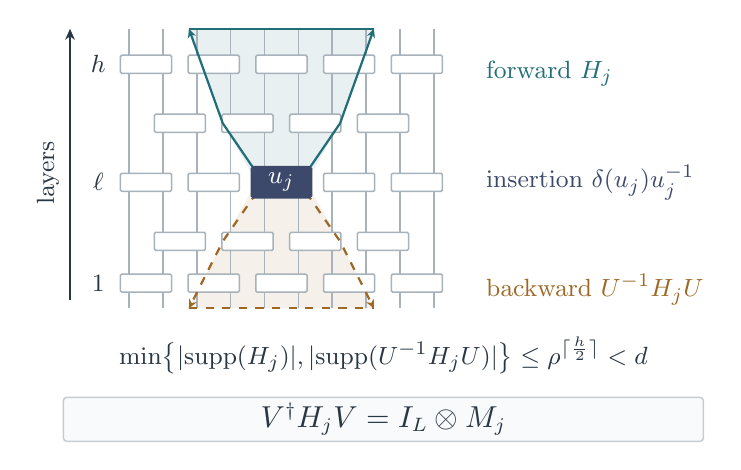
\begin{tikzpicture}[
 x=1cm,y=1cm,font=\fontsize{9.5}{11}\selectfont,text=FOneInk,
 f1wire/.style={draw=FOneWire,line width=0.55pt},
 f1brick/.style={draw=FOneWire,line width=0.55pt,fill=white,
   rounded corners=0.5pt},
 f1tree/.style={draw=FOneTeal,line width=0.65pt},
 f1clifford/.style={draw=FOneTeal,line width=0.65pt,
   fill=FOneTeal!13,rounded corners=0.7pt,
   minimum width=0.39cm,minimum height=0.25cm,inner sep=0pt},
 f1brace/.style={draw=FOneInk,line width=0.6pt,
   decorate,decoration={brace,amplitude=3.5pt}},
 f1footer/.style={draw=FOneWire!65,line width=0.55pt,
   fill=FOneNavy!3,rounded corners=1.3pt,minimum height=0.56cm,
   inner xsep=5pt,inner ysep=2pt},
 f1panel/.style={anchor=west,font=\bfseries\fontsize{10}{11.5}\selectfont}
]
% (a) Gate insertion in a schematic circuit; time runs upward.
\path[fill=FOneTeal,fill opacity=0.10]
 (2.67,3.40)--(2.24,4.15)--(1.81,5.35)--(4.16,5.35)
 --(3.73,4.15)--(3.30,3.40)--cycle;
\path[fill=FOneAmber,fill opacity=0.10]
 (2.67,3.40)--(2.24,2.65)--(1.81,1.80)--(4.16,1.80)
 --(3.73,2.65)--(3.30,3.40)--cycle;
\foreach \i in {0,...,9}{
 \pgfmathsetmacro{\wx}{1.05+0.43*\i}
 \draw[f1wire] (\wx,1.80)--(\wx,5.35);
}
\foreach \yy in {2.12,3.40,4.90}{
 \foreach \i in {0,2,4,6,8}{
  \pgfmathsetmacro{\xa}{0.94+0.43*\i}
  \pgfmathsetmacro{\xb}{1.59+0.43*\i}
  \draw[f1brick] (\xa,\yy-0.115) rectangle (\xb,\yy+0.115);
 }
}
\foreach \yy in {2.65,4.15}{
 \foreach \i in {1,3,5,7}{
  \pgfmathsetmacro{\xa}{0.94+0.43*\i}
  \pgfmathsetmacro{\xb}{1.59+0.43*\i}
  \draw[f1brick] (\xa,\yy-0.115) rectangle (\xb,\yy+0.115);
 }
}
\draw[FOneTeal,line width=0.8pt,-{Stealth[length=3.2pt,width=3pt]}]
 (2.67,3.52)--(2.24,4.15)--(1.81,5.35);
\draw[FOneTeal,line width=0.8pt,-{Stealth[length=3.2pt,width=3pt]}]
 (3.30,3.52)--(3.73,4.15)--(4.16,5.35);
\draw[FOneTeal,line width=0.8pt] (1.81,5.35)--(4.16,5.35);
\draw[FOneAmber,line width=0.8pt,dashed,
 -{Stealth[length=3.2pt,width=3pt]}]
 (2.67,3.27)--(2.24,2.65)--(1.81,1.80);
\draw[FOneAmber,line width=0.8pt,dashed,
 -{Stealth[length=3.2pt,width=3pt]}]
 (3.30,3.27)--(3.73,2.65)--(4.16,1.80);
\draw[FOneAmber,line width=0.8pt,dashed] (1.81,1.80)--(4.16,1.80);
\node[draw=FOneNavy,fill=FOneNavy,text=white,line width=0.7pt,
 rounded corners=0.7pt,minimum width=0.76cm,minimum height=0.39cm,
 inner sep=0pt] at (2.985,3.40) {\(u_j\)};
\draw[FOneInk,line width=0.6pt,-{Stealth[length=4pt,width=3.5pt]}]
 (0.30,1.91)--(0.30,5.35);
\node[rotate=90,font=\fontsize{9}{10}\selectfont] at (0.02,3.52) {layers};
\node at (0.66,2.12) {\(1\)};
\node at (0.66,3.40) {\(\ell\)};
\node at (0.66,4.90) {\(h\)};
\node[anchor=west,align=left,text=FOneTeal] at (5.46,4.78)
 {forward \(H_j\)};
\node[anchor=west,align=left,text=FOneNavy] at (5.46,3.40)
 {insertion \(\delta(u_j)u_j^{-1}\)};
\node[anchor=west,align=left,text=FOneAmber] at (5.46,2.04)
 {backward \(U^{-1}H_jU\)};
\node[inner sep=0pt] at (4.28,1.20)
 {\(\min\!\left\{
    \lvert\operatorname{supp}(H_j)\rvert,
   \lvert\operatorname{supp}(U^{-1}H_jU)\rvert
   \right\}\le \rho^{\lceil \frac{h}{2}\rceil}<d\)};
\node[f1footer,minimum width=8.13cm,
 font=\fontsize{10.5}{12}\selectfont] at (4.28,0.39)
 {\(V^\dagger H_jV=I_L\otimes M_j\)};

\end{tikzpicture}%
}
\caption{Two-sided light cones. A derivation applied to gate \(u_j\) in layer \(\ell\) gives the propagated
insertion \(H_j\). Under the depth condition, its forward support or
the backward support of \(U^{-1}H_jU\) is detectable.
Error detection and the exact encoded action yield gauge-only
compression of \(H_j\) in the output frame.
The brickwall arrangement assumes no geometric locality.}
\label{fig:mechanisms}
\end{figure}

\begin{samepage}
\begin{theorem}\label{thm:depth}
Let $n,h\ge 1$, and \(\rho\ge2\) be integers, and let
\(V\) encode a quantum code \(\mathcal C\) satisfying Eq.~\eqref{eq:correctable}
for a distance \(d\ge2\) on \(n\) physical subsystems. If
\begin{equation}\label{eq:depth}
  h<2\lceil\log_{\rho} d\rceil-1,
\end{equation}
then the logical actions of all circuits of depth at most \(h\), with gates
on at most \(\rho\) subsystems, that satisfy Eq.~\eqref{eq:encoded} obey
\[
 |\mathcal L_{\le h}(\mathcal C,\rho)|<\infty.
\]
All gate supports and unitary matrices are allowed. Consequently,
\(\mathcal L_{\le h}(\mathcal C,\rho)\) is not dense in \(\PU(K)\).
\end{theorem}
\end{samepage}

\begin{proof}
We fix a support arrangement and show that its circuits give finitely
many logical conjugation matrices. The entries of these matrices are
polynomial coordinates once we introduce variables for the gate and
encoded inverses. We will show that every derivation over \(\mathbb C\)
annihilates these coordinates at each field-valued solution, so that
Lemma~\ref{lem:algebraic-finite-image} applies.

We first define the circuit parameters and the logical conjugation coordinates.
Pad to \(h\) layers and \(n\) slots per layer, using identity gates on
empty supports. Scalar gates on empty supports affect only the global
phase. There are finitely many ordered support arrangements \(\alpha\).
Fix one and label its \(J=nh\) slots in execution order. For a slot
with support \(S_j\), take two independent matrices on
\(\bigotimes_{i\in S_j}\HH_i\). Extend both by the identity on the
complement and call the resulting matrices \(u_j,v_j\). Write
\(U=u_J\cdots u_1\). Likewise, take \(K\times K\) matrices \(W,W'\)
and \(g\times g\) matrices \(Z,Z'\). Put \(E=V^\dagger\) and
\(Q=W\otimes Z\). The matrices \(V,E\) are constant and \(EV=\id_L\otimes\id_G\).

Let \(\mathbf x\) consist of the entries of the local matrices and
of \(W,W',Z,Z'\). The coordinate algebra \(R_\alpha=\mathbb C[\mathbf x]/I_\alpha\)
is defined by the entrywise relations
\begin{align}
 u_jv_j=v_ju_j&=\id,\nonumber\\
 WW'=W'W&=\id_L,\quad ZZ'=Z'Z=\id_G,\label{eq:algebraic-inverses}\\
 UV&=VQ,\qquad EU=QE.\label{eq:algebraic-encoding}
\end{align}
In particular \(v_j=u_j^{-1}\), \(W'=W^{-1}\), \(Z'=Z^{-1}\), and
\(Q^{-1}=W'\otimes Z'\). Each physical circuit gives an evaluation
\(R_\alpha\to\mathbb C\), using adjoints for these inverses. Indeed,
\(UV=VQ\) implies \(U^{-1}V=VQ^{-1}\). At a physical evaluation
\(U\) and \(Q\) are unitary, so taking adjoints gives \(EU=QE\).

For \(1\le a,b,c,e\le K\), define in \(R_\alpha\)
\begin{equation}\label{eq:conjugation-coordinates}
 r_{abce}=W_{ab}W'_{ce}.
\end{equation}
This is the \((a,e)\) entry of \(W\mathsf e_{bc}W'\), where
\(\mathsf e_{bc}\) is the logical matrix unit with its only nonzero
entry at \((b,c)\). These \(K^4\) coordinates determine the
conjugation map \(X\mapsto WXW^{-1}\).

We next bound the support of each differentiated gate in both circuit directions.
Fix a field extension \(F/\mathbb C\), a \(\mathbb C\)-algebra map
\(\phi:R_\alpha\to F\), and a \(\mathbb C\)-linear derivation
\(\delta:F\to F\). Below the same symbols denote the evaluated
matrices. The rule \(\delta(xy)=\delta(x)y+x\delta(y)\) extends to
matrix products by applying \(\delta\) entrywise. The relations above
use matrix inverses over \(F\). For any supported operator over \(F\)
write \(O=\sum_\mu a_\mu B_\mu\), where the \(B_\mu\) are local
complex matrix units extended by identities. If the support has
size less than \(d\), Eq.~\eqref{eq:correctable} gives
\(EOV=\id_L\otimes\sum_\mu a_\mu M_{B_\mu}\). This is the detection
identity over \(F\).

Put \(U_{>j}=u_J\cdots u_{j+1}\) and \(U_{<j}=u_{j-1}\cdots u_1\),
with an empty product equal to the identity. The product rule gives
\[
 \delta(U)=\sum_{j=1}^J U_{>j}\delta(u_j)U_{<j}.
\]
In the \(j\)th term of \(\delta(U)U^{-1}\), write
\(U^{-1}=U_{<j}^{-1}u_j^{-1}U_{>j}^{-1}\).
The adjacent factors \(U_{<j}U_{<j}^{-1}\) cancel, giving
\begin{equation}\label{eq:generator}
 \begin{aligned}
 H&=\delta(U)U^{-1}=\sum_{j=1}^J H_j,\\
 H_j&=U_{>j}\delta(u_j)u_j^{-1}U_{>j}^{-1}.
 \end{aligned}
\end{equation}
In the input frame, substituting \(U=U_{>j}u_jU_{<j}\) cancels
the factors \(U_{>j}\) and \(U_{>j}^{-1}\), leaving
\[
 \begin{aligned}
 U^{-1}H_jU
 &=U_{<j}^{-1}u_j^{-1}\bigl(\delta(u_j)u_j^{-1}\bigr)u_jU_{<j}\\
 &=U_{<j}^{-1}u_j^{-1}\delta(u_j)U_{<j}.
 \end{aligned}
\]
Both local products \(\delta(u_j)u_j^{-1}\) and \(u_j^{-1}\delta(u_j)\)
are supported on \(S_j\). Other gates in the same layer are
disjoint from \(S_j\). Each later or earlier layer enlarges the
support by at most a factor \(\rho\). For slot \(j\) in layer
\(\ell\), the output and input support bounds are therefore
\(\rho^{h-\ell+1}\) and \(\rho^\ell\), respectively (Fig.~\ref{fig:mechanisms}).
The smaller is at most \(\rho^{\lceil \frac{h}{2}\rceil}\), since
\(\min\{h-\ell+1,\ell\}\le\lceil\frac{h}{2}\rceil\).
By Eq.~\eqref{eq:depth}, \(\lceil\frac{h}{2}\rceil\le
\lceil\log_\rho d\rceil-1<\log_\rho d\), so this support has size
less than \(d\).

We use error detection to compress each term and isolate the logical factor.
If the output support is detectable, Eq.~\eqref{eq:correctable}
gives \(EH_jV=\id_L\otimes M_j\) directly. Otherwise detection in
the input frame gives \(EU^{-1}H_jUV=\id_L\otimes N_j\).
Using \(EU^{-1}=Q^{-1}E\) and \(UV=VQ\) from
Eq.~\eqref{eq:algebraic-encoding}, we obtain
\begin{align*}
 EU^{-1}H_jUV&=Q^{-1}(EH_jV)Q,\\
 EH_jV&=Q(\id_L\otimes N_j)Q^{-1}
       =\id_L\otimes ZN_jZ^{-1}.
\end{align*}
Thus in either case \(EH_jV=\id_L\otimes M_j\) in the output
frame. Summing over \(j\), we have
\begin{equation}\label{eq:compression}
 EHV=\id_L\otimes M,\qquad M=\sum_{j=1}^J M_j.
\end{equation}

Since \(V,E\) are constant, differentiating \(UV=VQ\) gives
\(\delta(U)V=V\delta(Q)\). With \(U^{-1}V=VQ^{-1}\), this yields
\[
 EHV=E\delta(U)VQ^{-1}
     =EV\delta(Q)Q^{-1}
     =\delta(Q)Q^{-1}.
\]
Applying the product rule to \(Q=W\otimes Z\) gives
\(\delta(Q)=\delta(W)\otimes Z+W\otimes\delta(Z)\). Set
\(A_L=\delta(W)W^{-1}\) and \(B_G=\delta(Z)Z^{-1}\).
Multiplying \(\delta(Q)\) on the right by
\(Q^{-1}=W^{-1}\otimes Z^{-1}\) gives
\begin{equation}\label{eq:logicalgen}
 \delta(Q)Q^{-1}=A_L\otimes\id_G+\id_L\otimes B_G.
\end{equation}
Comparison with Eq.~\eqref{eq:compression} gives
\(A_L\otimes\id_G=\id_L\otimes(M-B_G)\). Taking the \((1,1)\)
matrix entry in the gauge factor on both sides leaves
\(A_L=\lambda\id_L\), with \(\lambda=(M-B_G)_{11}\in F\).

We now show that the conjugation coordinates have zero derivative and apply the finite-image lemma.
It follows that \(\delta(W)=\lambda W\). Differentiating \(WW'=\id_L\)
and multiplying on the left by \(W'\) gives
\(\delta(W')=-W'\delta(W)W'=-\lambda W'\).
Hence the two terms in the derivative of each conjugation coordinate
cancel:
\[
 \begin{aligned}
 \delta(r_{abce})&=\delta(W_{ab})W'_{ce}+W_{ab}\delta(W'_{ce})\\
                 &=\lambda W_{ab}W'_{ce}-W_{ab}\lambda W'_{ce}=0.
 \end{aligned}
\]
In particular, we can take \(F=\operatorname{Frac}(R_\alpha/\mathfrak p)\)
and \(\phi\) the canonical map for any minimal prime \(\mathfrak p\).
The hypothesis of Lemma~\ref{lem:algebraic-finite-image} is therefore
satisfied, and the joint evaluation image of the coordinates is finite.

If two physical evaluations yield the same conjugation matrix,
\(W_2^{-1}W_1\) commutes with every logical matrix unit. Commutation with
the diagonal units makes it diagonal, and commutation with the
off-diagonal units makes all its diagonal entries equal.
Since \(W_1,W_2\) are unitary, this common scalar has modulus one.
Each coordinate tuple thus determines at most one projective logical
action. The union over the finitely many support arrangements is
finite, and it cannot be dense in \(\PU(K)\) for \(K\ge2\).
\end{proof}


Finiteness does not exclude a finite subset \(S\subseteq\mathcal L_{\le h}(\mathcal C,\rho)\)
for which
\[
 \overline{\langle S\rangle}=\PU(K).
\]
The group \(\langle S\rangle\) allows words of arbitrary finite length.
A word of length \(r\) in \(S\cup S^{-1}\) has a concatenated
implementation of depth at most \(rh\). These products are not required
to remain in \(\mathcal L_{\le h}(\mathcal C,\rho)\), so density of the generated group does not
assert density within the original depth bound.
For example, Dua et al.\ give a \([[37,1,7]]\) CSS code with separate depth-one
circuits of gate range \(\rho=3\) that
implement~\cite[Sec.~V and Appendix~B~3]{Dua}
\[
 S=\bigl\{\overline T^\dagger,
          \sqrt{\overline X}^{\,\dagger}\bigr\}
   \subseteq\mathcal L_{\le1}(\mathcal C,3).
\]
The two circuits use different partitions of the physical qubits.
Since \(\overline H\propto
(\overline T^\dagger)^2\sqrt{\overline X}^{\,\dagger}
(\overline T^\dagger)^2\) and
\(\overline T=(\overline T^\dagger)^7\), this pair generates a dense
subgroup of \(\PU(2)\). For this code,
\(2\lceil\log_3 7\rceil-1=3\), so \(\mathcal L_{\le1}(\mathcal C,3)\) is finite by
Theorem~\ref{thm:depth}.


In a fault-tolerance threshold construction based on the constant-depth
unitary logical gadgets considered here, logical-gate compilation is
necessary for universal control in the finite-image regime. On a fixed
code, the available shallow logical actions form a finite alphabet. If
its generated group is dense, arbitrary target logical unitaries can be
approximated by words over this alphabet, with error correction
interleaved as prescribed by the protocol~\cite{Gottesman,Dua}. The
constant-depth premise applies to each gadget. Compiled word lengths cannot
remain uniformly bounded when arbitrary targets must be approximated to
arbitrarily high accuracy.

The finiteness condition has an exact boundary for stabilizer codes. For an integer \(\rho\ge2\), define the critical depth
\begin{equation}\label{eq:critical-definition}
 h_\infty(\mathcal C,\rho)
  =\min\{h\in\mathbb Z_{\ge1}:\mathcal L_{\le h}(\mathcal C,\rho)
                   \text{ is infinite}\},
\end{equation}
with value \(\infty\) if the set is empty. When \(d\ge2\), Theorem~\ref{thm:depth} gives
\begin{equation}\label{eq:critical-lower}
 h_\infty(\mathcal C,\rho)\ge2\lceil\log_{\rho} d\rceil-1.
\end{equation}

For the upper bound of $h_\infty(\mathcal C,\rho)$, we implement continuous
rotations generated by a weight-\(d\) logical Pauli. A Clifford tree
collects its nonidentity factors onto at most \(\rho\) qubits in
\(\lceil\log_\rho d\rceil-1\) layers. The compressed Pauli then fits
in one allowed rotation gate. Conjugating back recovers the original
Pauli rotation, at total depth \(2\lceil\log_\rho d\rceil-1\).
This uses the established tree constructions for parity compression,
phase gadgets, and Pauli-rotation
synthesis~\cite{BonetMonroig,Cowtan,HaahLiuTan}.
The resulting continuous family is nonconstant modulo phase, giving
the matching upper bound.

\begin{figure}[!ht]
\centering
\resizebox{\columnwidth}{!}{%
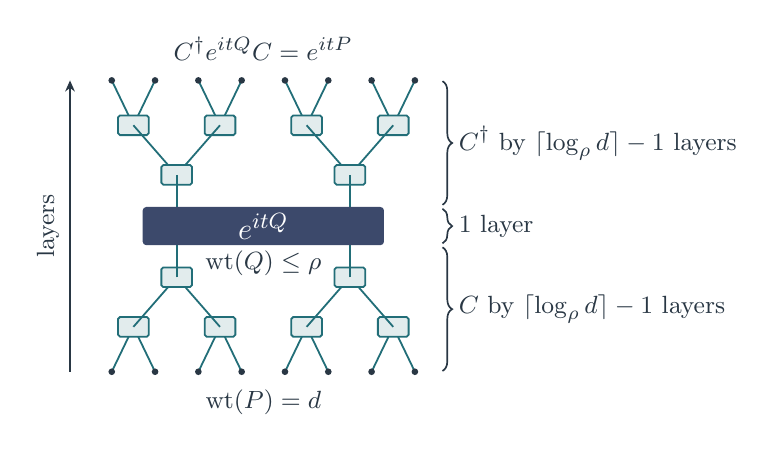
\begin{tikzpicture}[
 x=1cm,y=1cm,font=\fontsize{9.5}{11}\selectfont,text=FOneInk,
 f1wire/.style={draw=FOneWire,line width=0.55pt},
 f1brick/.style={draw=FOneWire,line width=0.55pt,fill=white,
   rounded corners=0.5pt},
 f1tree/.style={draw=FOneTeal,line width=0.65pt},
 f1clifford/.style={draw=FOneTeal,line width=0.65pt,
   fill=FOneTeal!13,rounded corners=0.7pt,
   minimum width=0.39cm,minimum height=0.25cm,inner sep=0pt},
 f1brace/.style={draw=FOneInk,line width=0.6pt,
   decorate,decoration={brace,amplitude=3.5pt}},
 f1footer/.style={minimum height=0.56cm,
   inner xsep=5pt,inner ysep=2pt},
 f1panel/.style={anchor=west,font=\bfseries\fontsize{10}{11.5}\selectfont}
]
\begin{scope}[xshift=-9cm]
% (b) Active Pauli support only. Binary branching illustrates the \rho-ary tree.
\draw[FOneInk,line width=0.6pt,-{Stealth[length=4pt,width=3.5pt]}]
 (9.72,1.60)--(9.72,5.30);
\node[rotate=90,font=\fontsize{9}{10}\selectfont] at (9.44,3.45) {layers};
\node at (12.175,5.70) {\(C^\dagger e^{itQ}C=e^{itP}\)};
\node at (12.175,1.21) {\(\operatorname{wt}(P)=d\)};
\foreach \sgn in {-1,1}{
 \pgfmathsetmacro{\yl}{3.45+\sgn*1.85}
 \pgfmathsetmacro{\yone}{3.45+\sgn*1.28}
 \pgfmathsetmacro{\ytwo}{3.45+\sgn*0.65}
 \pgfmathsetmacro{\yg}{3.45+\sgn*0.23}
 \foreach \xa/\xb/\xc in {
 10.25/10.80/10.525,11.35/11.90/11.625,
 12.45/13.00/12.725,13.55/14.10/13.825}{
  \draw[f1tree] (\xa,\yl)--(\xc,\yone);
  \draw[f1tree] (\xb,\yl)--(\xc,\yone);
  \node[f1clifford] at (\xc,\yone) {};
 }
 \foreach \xa/\xb/\xc in {10.525/11.625/11.075,12.725/13.825/13.275}{
  \draw[f1tree] (\xa,\yone)--(\xc,\ytwo);
  \draw[f1tree] (\xb,\yone)--(\xc,\ytwo);
  \node[f1clifford] at (\xc,\ytwo) {};
  \draw[f1tree] (\xc,\ytwo)--(\xc,\yg);
 }
 \foreach \xx in {10.25,10.80,11.35,11.90,12.45,13.00,13.55,14.10}{
  \fill[FOneInk] (\xx,\yl) circle (1.2pt);
 }
}
\node at (12.175,2.98) {\(\operatorname{wt}(Q)\le \rho\)};
\node[draw=FOneNavy,fill=FOneNavy,text=white,line width=0.7pt,
 rounded corners=1pt,minimum width=3.04cm,minimum height=0.46cm,
 inner sep=0pt,font=\fontsize{11}{12}\selectfont] at (12.175,3.45)
 {\(e^{itQ}\)};
\draw[f1brace] (14.45,3.18)--(14.45,1.61);
\node[anchor=west,align=left,inner xsep=0pt] at (14.65,2.395)
 {\(C\) by \(\lceil\log_\rho d\rceil-1\) layers};
\draw[f1brace] (14.45,3.67)--(14.45,3.23);
\node[anchor=west,inner xsep=0pt] at (14.65,3.45) {1 layer};
\draw[f1brace] (14.45,5.29)--(14.45,3.72);
\node[anchor=west,align=left,inner xsep=0pt] at (14.65,4.505)
 {\(C^\dagger\) by \(\lceil\log_\rho d\rceil-1\) layers};
\end{scope}
\end{tikzpicture}%
}
\caption{Mechanism of Theorem~\ref{cor:critical}. Time runs upward.
\(C\) compresses the support of a
weight-\(d\) logical Pauli to \(Q=CPC^\dagger\), with
\(\operatorname{wt}(Q)\le\rho\). One rotation gate followed by
\(C^\dagger\) gives the complete logical circuit
\(C^\dagger e^{itQ}C=e^{itP}\), of depth \(2\lceil\log_\rho d\rceil-1\).}
\label{fig:pauli-compression}
\end{figure}

\begin{samepage}
\begin{theorem}\label{cor:critical}
Let \(\mathcal C\) be an \([[n,k,d]]\) qubit stabilizer code,
with \(k\ge1\) and actual distance \(d\ge2\). Let \(\rho\ge2\) be an
integer, and allow arbitrary unitary gates on any set of at most \(\rho\)
qubits. Then
\begin{equation}\label{eq:critical}
 h_\infty(\mathcal C,\rho)=2\lceil\log_{\rho} d\rceil-1.
\end{equation}
At this depth, the logical image contains a nontrivial continuous
one-parameter subgroup.
\end{theorem}
\end{samepage}

\begin{proof}
Put \(m=\lceil\log_\rho d\rceil\). It suffices to construct infinitely many
logical actions at depth at most \(2m-1\).
Choose a Hermitian code-preserving Pauli \(P\) of weight \(d\), with
\(P^2=\id\) and nonscalar logical action
\(\overline P\)~\cite[Sec.~3.2]{GottesmanStabilizer}.
We first compress its support so that its rotation fits in one allowed
gate.

We adapt the unitary parity-concentration part of the binary-tree
in-line symmetry-verification circuit in
Ref.~\cite[Sec.~IV and Fig.~2(a)]{BonetMonroig}
to gates on at most \(\rho\) qubits.
At each layer, partition the active factors into groups of \(\rho\),
with at most one smaller group. In each group, basis changes and CNOTs
compose into one allowed Clifford gate collecting the product onto
one qubit. The disjoint groups form one layer.
If \(w_r\) is the weight after \(r\) layers, then
\(w_0=d\) and \(w_{r+1}=\lceil\frac{w_r}{\rho}\rceil\), giving
\(w_r=\lceil\frac{d}{\rho^r}\rceil\).
Thus \(m-1\) layers yield \(C\) with \(Q=CPC^\dagger\) of weight at
most \(\rho\). 
The compressed rotation \(e^{itQ}\) is one allowed gate.
Conjugating back gives
\begin{equation}\label{eq:pauli-family}
 U(t)=C^\dagger e^{itQ}C=e^{itP}.
\end{equation}
The depth is at most \((m-1)+1+(m-1)=2m-1\).
The complete circuit preserves the code and induces
\(e^{it\overline P}\). As \(\overline P\) has both eigenvalues
\(\pm1\), its projective rotations form a nontrivial continuous
\(\mathrm U(1)\) subgroup of period \(\pi\).
Hence \(h_\infty(\mathcal C,\rho)\le2m-1\), and the lower bound gives
Eq.~\eqref{eq:critical}.
\end{proof}
The construction attains the threshold for an infinite exact logical image,
but does not by itself provide fault tolerance against arbitrary single-gate faults.
An error \(e^{i\varepsilon Q}\) immediately after the central rotation gate
propagates through \(C^\dagger\) to \(e^{i\varepsilon P}\), which induces
a nontrivial logical error for \(\varepsilon\notin\pi\mathbb Z\).

\textit{Conclusion.}
For general quantum codes in the finite-dimensional setting considered
here, bounded-range circuits below the stated threshold realize only
finitely many exact logical actions up to phase. The proof combines a
detectable light cone in one of the two circuit directions with a
finite-image criterion for the circuit coordinate algebra.
Qubit stabilizer codes attain the bound by concentrating the support
of a logical Pauli into one rotation gate and then reversing the
compression. Together, the theorems locate the critical circuit depth to support
infinitely many exact logical actions without imposing geometric
locality.

\begin{acknowledgments}
\textit{*Acknowledgement.*} We acknowledge the use of ChatGPT 6.1 Sol to assist the preparation of this manuscript. Story unfolding is supported in part
by NSFC under Grant No. 12475023, Dushi Program, and a startup funding from YMSC.
\end{acknowledgments}

Lean proofs of the statements of Theorems~\ref{thm:depth}
and~\ref{cor:critical}, together with verification scripts, are available
in the \href{https://github.com/Imine20/critical-depth-for-the-infinite-logical-set/tree/ad6a378f6080ba32d92e7c31b6cf71b07685970a}{project repository}
(proof snapshot \texttt{ad6a378}). The proof of
Theorem~\ref{thm:depth} follows the coordinate-algebra and derivation
argument presented here, including scalar extension of detection,
two-sided support bounds and the finite-evaluation-image criterion.
The audited theorem dependencies contain no project axioms or
\texttt{sorryAx}; their foundational axioms are
\texttt{propext}, \texttt{Classical.choice} and \texttt{Quot.sound}.
The quantitative bounds and computational discussion in the End Matter
are additional mathematical deductions and are not formalized in this
snapshot.

\begin{thebibliography}{18}
\rightskip=0pt plus 1fil\relax
\bibitem{Gottesman}
D.~Gottesman,
\href{https://doi.org/10.26421/QIC14.15-16-5}
{Quantum Inf.\ Comput.\ \textbf{14}, 1338--1371 (2014)},
\href{https://arxiv.org/abs/1310.2984}{arXiv:1310.2984}.

\bibitem{EK}
B.~Eastin and E.~Knill,
\href{https://doi.org/10.1103/PhysRevLett.102.110502}
{Phys.\ Rev.\ Lett.\ \textbf{102}, 110502 (2009)},
\href{https://arxiv.org/abs/0811.4262}{arXiv:0811.4262}.

\bibitem{BK}
S.~Bravyi and R.~K\"onig,
\href{https://doi.org/10.1103/PhysRevLett.110.170503}
{Phys.\ Rev.\ Lett.\ \textbf{110}, 170503 (2013)},
\href{https://arxiv.org/abs/1206.1609}{arXiv:1206.1609}.

\bibitem{PY}
F.~Pastawski and B.~Yoshida,
\href{https://doi.org/10.1103/PhysRevA.91.012305}
{Phys.\ Rev.\ A \textbf{91}, 012305 (2015)},
\href{https://arxiv.org/abs/1408.1720}{arXiv:1408.1720}.

\bibitem{JKY}
T.~Jochym-O'Connor, A.~Kubica, and T.~J.~Yoder,
\href{https://doi.org/10.1103/PhysRevX.8.021047}
{Phys.\ Rev.\ X \textbf{8}, 021047 (2018)},
\href{https://arxiv.org/abs/1710.07256}{arXiv:1710.07256}.

\bibitem{Webster}
P.~Webster, M.~Vasmer, T.~R.~Scruby, and S.~D.~Bartlett,
\href{https://doi.org/10.1103/PhysRevResearch.4.013092}
{Phys.\ Rev.\ Research \textbf{4}, 013092 (2022)},
\href{https://arxiv.org/abs/2012.05260}{arXiv:2012.05260}.

\bibitem{KL}
E.~Knill and R.~Laflamme,
\href{https://doi.org/10.1103/PhysRevA.55.900}
{Phys.\ Rev.\ A \textbf{55}, 900 (1997)},
\href{https://arxiv.org/abs/quant-ph/9604034}{arXiv:quant-ph/9604034}.

\bibitem{Kribs}
D.~Kribs, R.~Laflamme, and D.~Poulin,
\href{https://doi.org/10.1103/PhysRevLett.94.180501}
{Phys.\ Rev.\ Lett.\ \textbf{94}, 180501 (2005)},
\href{https://arxiv.org/abs/quant-ph/0412076}{arXiv:quant-ph/0412076}.

\bibitem{Faist}
P.~Faist, S.~Nezami, V.~V.~Albert, G.~Salton, F.~Pastawski,
P.~Hayden, and J.~Preskill,
\href{https://doi.org/10.1103/PhysRevX.10.041018}
{Phys.\ Rev.\ X \textbf{10}, 041018 (2020)},
\href{https://arxiv.org/abs/1902.07714}{arXiv:1902.07714}.

\bibitem{LiuZhou}
Z.-W.~Liu and S.~Zhou,
\href{https://doi.org/10.1038/s41534-023-00788-4}
{npj Quantum Inf.\ \textbf{9}, 119 (2023)},
\href{https://arxiv.org/abs/2111.06355}{arXiv:2111.06355}.
See also its long supplement,
\href{https://arxiv.org/abs/2111.06360}{arXiv:2111.06360}, Sec.~VI.

\bibitem{Dua}
A.~Dua, A.~Holmes, M.~J.~Gullans, and V.~V.~Albert,
\emph{Qubit CSS codes with Universal Transversal Gates},
\href{https://arxiv.org/abs/2610.06730v1}{arXiv:2610.06730v1} (2026).

\bibitem{BonetMonroig}
X.~Bonet-Monroig, R.~Sagastizabal, M.~Singh, and T.~E.~O'Brien,
\href{https://doi.org/10.1103/PhysRevA.98.062339}
{Phys.\ Rev.\ A \textbf{98}, 062339 (2018)},
\href{https://arxiv.org/abs/1807.10050}{arXiv:1807.10050}.

\bibitem{Cowtan}
A.~Cowtan, S.~Dilkes, R.~Duncan, W.~Simmons, and S.~Sivarajah,
\href{https://doi.org/10.4204/EPTCS.318.13}
{Electron.\ Proc.\ Theor.\ Comput.\ Sci.\ \textbf{318}, 213 (2020)},
\href{https://arxiv.org/abs/1906.01734}{arXiv:1906.01734}.

\bibitem{HaahLiuTan}
J.~Haah, Y.~Liu, and X.~Tan,
\href{https://doi.org/10.1007/s00220-025-05480-6}
{Commun.\ Math.\ Phys.\ \textbf{406}, 309 (2025)},
\href{https://arxiv.org/abs/2402.05239}{arXiv:2402.05239}.

\bibitem{GottesmanStabilizer}
D.~Gottesman,
\emph{Stabilizer Codes and Quantum Error Correction},
Ph.D. thesis, California Institute of Technology (1997),
\href{https://arxiv.org/abs/quant-ph/9705052}{arXiv:quant-ph/9705052}.

\bibitem{Stacks}
The Stacks Project Authors,
\href{https://stacks.math.columbia.edu/tag/00FR}{Lemma 10.31.6 (Tag 00FR)}
and \href{https://stacks.math.columbia.edu/tag/00E0}{Lemma 10.17.2 (Tag 00E0)},
\emph{The Stacks Project}.

\bibitem{BurgisserScheiblechner}
P.~B\"urgisser and P.~Scheiblechner,
\emph{On the complexity of counting components of algebraic varieties},
\href{https://doi.org/10.1016/j.jsc.2008.02.009}{J.~Symbolic Comput.\ \textbf{44}, 1114--1136 (2009)};
\href{https://www.scheiblechner.ch/files/count-comp.pdf}{author manuscript},
Secs.~2.1.2--2.1.3.

\bibitem{BasuPollackRoy}
S.~Basu, R.~Pollack, and M.-F.~Roy,
\href{https://doi.org/10.1007/3-540-33099-2}
{\emph{Algorithms in Real Algebraic Geometry}},
2nd ed. (Springer, Berlin, 2006).

\end{thebibliography}

\section*{End Matter}
\subsection*{Algebraic finite-image criterion}

We give the global finiteness step in detail. The objects of interest
are finitely many elements \(r_1,\ldots,r_m\) of a coordinate algebra
\(R\), representing the output coordinates of a polynomial map.
An evaluation is a unital \(\mathbb C\)-algebra homomorphism
\(\phi:R\to\mathbb C\). We seek a finite set containing all output
tuples \((\phi(r_1),\ldots,\phi(r_m))\); neither the set of evaluations
nor the whole parameter space is required to be finite.

For a minimal prime ideal \(\mathfrak p\) of \(R\), put
\[
 F_{\mathfrak p}=\operatorname{Frac}(R/\mathfrak p),\qquad
 \iota_{\mathfrak p}:R\longrightarrow R/\mathfrak p
                         \longrightarrow F_{\mathfrak p}.
\]
The quotient is an integral domain, so its map into its fraction
field is injective and \(\ker\iota_{\mathfrak p}=\mathfrak p\).
A \(\mathbb C\)-linear derivation \(\delta:F_{\mathfrak p}\to
F_{\mathfrak p}\) is a linear map satisfying
\(\delta(xy)=\delta(x)y+x\delta(y)\).
The derivations must be taken in these function fields: a
\(\mathbb C\)-linear derivation of \(\mathbb C\) itself is always zero
and would give no constraint on the outputs.

\begin{lemma}\label{lem:algebraic-finite-image}
Let \(R\) be a finitely generated commutative \(\mathbb C\)-algebra,
and let \(r_1,\ldots,r_m\in R\). Suppose that, for every minimal prime
\(\mathfrak p\) and every \(\mathbb C\)-linear derivation
\(\delta:F_{\mathfrak p}\to F_{\mathfrak p}\),
\[
 \delta\bigl(\iota_{\mathfrak p}(r_i)\bigr)=0
 \quad\text{for every }i.
\]
Then the joint evaluation image
\[
 \{(\phi(r_1),\ldots,\phi(r_m)):
          \phi:R\to\mathbb C\text{ a }\mathbb C\text{-algebra map}\}
\]
is finite.
\end{lemma}

\begin{proof}
If \(R=0\), there is no unital map \(R\to\mathbb C\), and the image
is empty. Assume \(R\ne0\).

\emph{Constants in a function field.}
We first explain why an element \(a\) of a field extension
\(F/\mathbb C\) that is killed by every \(\mathbb C\)-linear
derivation must belong to \(\mathbb C\).
If \(a\) were transcendental, choose a transcendence basis \(B\) of
\(F/\mathbb C\) containing \(a\). On the rational function field
\(L=\mathbb C(B)\), partial differentiation with respect to \(a\)
defines a derivation with \(\delta(a)=1\), \(\delta(b)=0\) for
\(b\in B\setminus\{a\}\), and \(\delta(c)=0\) for \(c\in\mathbb C\).

The extension \(F/L\) is algebraic and, in characteristic zero,
separable. The derivation extends uniquely through this extension.
To see the mechanism, let \(\beta\) have minimal polynomial
\(f(T)=T^s+\sum_{j=0}^{s-1}a_jT^j\) over \(L\). Differentiating
\(f(\beta)=0\) forces
\[
 \delta(\beta)=-
 \frac{\sum_{j=0}^{s-1}\delta(a_j)\beta^j}{f'(\beta)}.
\]
Separability gives \(f'(\beta)\ne0\). For existence, extend
\(\delta\) from \(L\) to a derivation \(L[T]\to L(\beta)\), using
evaluation at \(\beta\) for the module structure and the displayed
value for \(\delta(T)\). The derivation kills \(f\), and the Leibniz
rule then makes it kill the whole ideal \((f)\). It descends to
\(L[T]/(f)=L(\beta)\), proving existence as well as uniqueness.
Extensions to finite intermediate fields agree on their overlaps,
so they define a derivation on \(F\). It still satisfies
\(\delta(a)=1\), contradicting the assumed vanishing.
Thus \(a\) is algebraic over \(\mathbb C\), and algebraic closedness
gives \(a\in\mathbb C\).

Apply this argument to \(F_{\mathfrak p}\). For each \(i,\mathfrak p\),
there is a constant \(c_{i,\mathfrak p}\in\mathbb C\) with
\(\iota_{\mathfrak p}(r_i)=c_{i,\mathfrak p}\).
The kernel calculation above therefore gives
\begin{equation}\label{eq:component-constants}
 r_i-c_{i,\mathfrak p}\in\mathfrak p.
\end{equation}
The same minimal prime supplies a whole constant output tuple.
At this stage we have a conclusion on each irreducible component;
we still need a finite number of components and control of every
evaluation, including points where components meet.

\emph{One polynomial for all evaluations.}
Hilbert's basis theorem makes \(R\) Noetherian. Hence its set of
minimal primes is finite and nonempty~\cite{Stacks}; write it as
\(\{\mathfrak p_1,\ldots,\mathfrak p_t\}\).
For each output coordinate form the monic polynomial
\[
 P_i(T)=\prod_{\nu=1}^{t}(T-c_{i,\mathfrak p_\nu}).
\]
For any \(\nu\), one factor of \(P_i(r_i)\) lies in
\(\mathfrak p_\nu\) by Eq.~\eqref{eq:component-constants}.
Consequently
\[
 P_i(r_i)\in
 \bigcap_{\nu=1}^{t}\mathfrak p_\nu=\sqrt{(0)}.
\]
The equality is the standard description of the nilradical as the
intersection of the minimal primes~\cite{Stacks}.
By definition of the nilradical, some positive integer \(a_i\)
satisfies \(P_i(r_i)^{a_i}=0\).
Thus \(r_i\) satisfies the monic polynomial \(P_i(T)^{a_i}\) in \(R\);
this is exactly the integrality statement used in the formal proof.
We have not assumed that \(R\) is reduced.

Now let \(\phi:R\to\mathbb C\) be \emph{any} evaluation.
Because \(\phi\) preserves the complex coefficients,
\[
 0=\phi\bigl(P_i(r_i)^{a_i}\bigr)
   =P_i\bigl(\phi(r_i)\bigr)^{a_i}.
\]
A field has no nonzero nilpotents, so \(P_i(\phi(r_i))=0\).
In particular, the same polynomial \(P_i\), chosen before \(\phi\),
constrains every value of the coordinate \(r_i\).
Its root set \(Z(P_i)\subset\mathbb C\) is finite since \(P_i\) is
nonzero. The joint evaluation image is contained in the finite product
\[
 Z(P_1)\times\cdots\times Z(P_m),
\]
which proves the lemma.
\end{proof}

Geometrically, the minimal primes describe the irreducible components
of the affine parameter space. The field-derivation calculation makes
each output coordinate constant on every such component, and
Noetherianity limits their number. The polynomial argument also
handles nilpotent directions: for example, in
\(R=\mathbb C[t,\epsilon]/(\epsilon^2)\), the element
\(r=\epsilon\) is nonzero but every complex evaluation sends it to
zero. The parameter \(t\) remains arbitrary. Thus a finite output
image does not imply that the coordinate algebra is reduced or that
its spectrum is zero-dimensional. No smoothness assumption or
restriction to regular points enters the argument.

For Theorem~\ref{thm:depth}, take \(R=R_\alpha\) and the \(K^4\)
coordinates in Eq.~\eqref{eq:conjugation-coordinates}.
The circuit calculation proves derivative vanishing for \emph{every}
field-valued solution, so in particular it applies to each canonical
map \(\iota_{\mathfrak p}\).
The lemma therefore gives a finite set containing the outputs of
all physical evaluations, including points on singular loci.
At a physical point the coordinates give \(A\mapsto WAW^\dagger\);
two such maps agree exactly when the two unitaries differ by a scalar
phase. Restricting the finite output image to physical evaluations
therefore proves finiteness of the required projective logical
actions for that support arrangement. This is the algebraic route
implemented in the cited Lean snapshot.

\subsection*{Quantitative parameters and exact counting}

The same component constants yield a cardinality bound. The kernel of
any evaluation \(R_\alpha\to\mathbb C\) contains a minimal prime
\(\mathfrak p\). All its logical conjugation coordinates therefore
have the single joint value \((c_{i,\mathfrak p})_i\). Hence
\begin{equation}\label{eq:component-bound}
 |\mathcal L_{\le h}(\mathcal C,\rho)|
 \le \sum_\alpha \#\operatorname{Min}(R_\alpha).
\end{equation}
Different components can give the same logical action, and some
algebraic solutions need not be physical, so equality is not asserted.

Here are explicit parameters for the presentation in the proof.
Write \(q_i=\dim\HH_i\), \(P=\prod_iq_i\), and
\(D_j=\prod_{i\in S_j}q_i\), taking \(D_j=1\) on empty supports.
With \(J=nh\) slots, the number of complex variables is
\begin{equation}\label{eq:coordinate-count}
 N_\alpha=2\sum_{j=1}^{J}D_j^2+2K^2+2g^2.
\end{equation}
There are at most
\(2JP^2+2K^2+2g^2+2PKg\) scalar defining relations, each of degree
at most \(\Delta=\max\{2,J\}\). The term \(2JP^2\) counts the two
inverse relations for each embedded physical gate; it is not an
optimized presentation. The affine B\'ezout bound, counting
irreducible components of all dimensions, gives
\(\#\operatorname{Min}(R_\alpha)\le\Delta^{N_\alpha}\)~\cite{BurgisserScheiblechner}.
Nilpotents do not add components or complex evaluations.

A support arrangement assigns each site in each layer either to one
of the \(n\) labelled slots or to no slot. There are therefore at most
\((n+1)^{nh}\) arrangements; disjointness and the arity restriction
only reduce this count. Set \(q_{\max}=\max_iq_i\) and
\(s=\min\{\rho,n\}\). Since \(D_j\le q_{\max}^{s}\), under the
hypotheses of Theorem~\ref{thm:depth} we obtain
\begin{equation}\label{eq:explicit-bound}
 \begin{gathered}
 |\mathcal L_{\le h}(\mathcal C,\rho)|
       \le (n+1)^{nh}\Delta^{N_*},\\
 N_*=2nh\,q_{\max}^{2s}+2K^2+2g^2,\qquad
 \Delta=\max\{2,nh\}.
 \end{gathered}
\end{equation}
This bound is uniform over encodings with these dimensions, but very
loose. For \(n=5\), \(h=\rho=2\), \(q_{\max}=K=2\), and \(g=1\),
it is \(6^{10}10^{330}\). A bound depending only on \(d,\rho,h\)
cannot hold across all codes: the \(k\)-fold tensor power of the
\([[5,1,3]]\) stabilizer code keeps \(d=3,\rho=2,h=1\), while its
depth-one logical image contains at least \(4^k\) projective logical
Paulis.

Exact counting requires more than a component bound. If the encoding
entries are supplied as exact algebraic numbers, introduce variables
\(y_i\) for the logical conjugation coordinates and eliminate all original
matrix-entry variables from \(I_\alpha+(y_i-r_i)_i\).
The resulting finite complex output variety gives candidate actions:
its image is already finite and thus Zariski closed.
For each candidate, retain its conjugation-coordinate equalities and
test the original unitary and encoding equations in real and imaginary
parts for solvability. Also,
duplicate actions from different components and arrangements must be
identified. Real quantifier elimination provides a decision procedure
for this feasibility step~\cite{BasuPollackRoy}. The inverse variables
of the enlarged complex model alone do not enforce physical unitarity.

These procedures are effective in principle with exact algebraic
input, but the variable count and elimination costs make direct
enumeration impractical in general. Arbitrary unspecified complex
encoding coefficients do not supply an effective input representation,
even though the theorem and Eq.~\eqref{eq:explicit-bound} still hold.
Exploiting symmetries, smaller presentations or a particular code may
improve the calculation. Equations~\eqref{eq:component-bound}--\eqref{eq:explicit-bound},
the B\'ezout estimate and the exact-counting procedure are not
formalized or executed by the cited Lean development.

\end{document}
